\documentclass[../../e3_tp3_main.tex]{subfiles}

\begin{document}

%capítulo
\chapter{}

The input of the system is $W$ and the output is $Z$. $Z=1$ if there has just been a transition from 0 to 1, and $Z=0$ otherwise. 

\section{Moore-type FSM implementation}
\subsection{FSM flow-chart}
\begin{figure}[H]
	\centering
	\begin{tikzpicture}
	\begin{pgfonlayer}{nodelayer}
		\node [style=estado] (0) at (0, 3) {Half full - pump: A};
		\node [style=estado] (1) at (0, -3) {Half full - pump: B};
		\node [style=estado] (2) at (9, 3) {Full - next pump: B};
		\node [style=estado] (3) at (9, -3) {Empty - next pump: B};
		\node [style=estado] (4) at (-9, -3) {Full - next pump: A};
		\node [style=estado] (5) at (-9, 3) {Empty - next pump: A};
		\node [style=none] (6) at (9, -3.75) {};
		\node [style=none] (7) at (0.5, -3.75) {};
		\node [style=none] (8) at (-0.5, -3.75) {};
		\node [style=none] (9) at (-9, -3.75) {};
		\node [style=none] (10) at (8.25, -4.5) {};
		\node [style=none] (11) at (1.25, -4.5) {};
		\node [style=none] (12) at (-1.25, -4.5) {};
		\node [style=none] (13) at (-8.25, -4.5) {};
		\node [style=none] (14) at (-9, 3.75) {};
		\node [style=none] (15) at (-0.5, 3.75) {};
		\node [style=none] (16) at (0.5, 3.75) {};
		\node [style=none] (17) at (9, 3.75) {};
		\node [style=none] (18) at (-8.25, 4.5) {};
		\node [style=none] (19) at (-1.25, 4.5) {};
		\node [style=none] (20) at (1.25, 4.5) {};
		\node [style=none] (21) at (8.25, 4.5) {};
		\node [style=none] (22) at (-10, -2.25) {};
		\node [style=none] (23) at (-9, -2.25) {};
		\node [style=none] (24) at (-10, 2.25) {};
		\node [style=none] (25) at (-9, 2.25) {};
		\node [style=none] (26) at (-8, 2.25) {};
		\node [style=none] (27) at (-8, -2.25) {};
		\node [style=none] (28) at (-0.5, -2.25) {};
		\node [style=none] (29) at (0.5, -2.25) {};
		\node [style=none] (30) at (-0.5, 2.25) {};
		\node [style=none] (31) at (0.5, 2.25) {};
		\node [style=none] (32) at (10, 2.25) {};
		\node [style=none] (33) at (9, 2.25) {};
		\node [style=none] (34) at (10, -2.25) {};
		\node [style=none] (35) at (9, -2.25) {};
		\node [style=none] (36) at (8, -2.25) {};
		\node [style=none] (37) at (8, 2.25) {};
	\end{pgfonlayer}
	\begin{pgfonlayer}{edgelayer}
		\draw [style=transicion] (24.center) to (22.center);
		\draw [style=transicion] (23.center) to (25.center);
		\draw [style=transicion] (34.center) to (32.center);
		\draw [style=transicion] (33.center) to (35.center);
		\draw [style=transicion, bend left=45] (16.center) to (20.center);
		\draw [style=transicion] (20.center) to (21.center);
		\draw [style=transicion, bend left=45] (21.center) to (17.center);
		\draw [style=transicion, bend left=45] (14.center) to (18.center);
		\draw [style=transicion] (18.center) to (19.center);
		\draw [style=transicion, bend left=45] (19.center) to (15.center);
		\draw [style=transicion, bend left=45] (8.center) to (12.center);
		\draw [style=transicion] (12.center) to (13.center);
		\draw [style=transicion, bend left=45] (13.center) to (9.center);
		\draw [style=transicion, bend left=45] (6.center) to (10.center);
		\draw [style=transicion] (10.center) to (11.center);
		\draw [style=transicion, bend left=45] (11.center) to (7.center);
		\draw [style=transicion, in=-90, out=90, looseness=0.75] (28.center) to (26.center);
		\draw [style=transicion, in=-90, out=90, looseness=0.75] (27.center) to (30.center);
		\draw [style=transicion, in=90, out=-90, looseness=0.75] (37.center) to (29.center);
		\draw [style=transicion, in=90, out=-90, looseness=0.75] (31.center) to (36.center);
	\end{pgfonlayer}
\end{tikzpicture}

	\caption{Flow diagram for the Moore-type FSM implementation.}
\end{figure}

\subsection{State descriptions}
\begin{table}[H]	%mealy state descriptions
	\centering
	\begin{tabular}{|c|c|}
	\hline	
	$y_0$, $y_1$  & Description\\	
	\hline 
	00 & The last number detected is a 0\\ 
	\hline 
	01 & The last two numbers detected were 0-1 (in order).\\ 
	\hline 
	10 & The last two numbers detected were 1-1.\\ 
	\hline
	
	\end{tabular} 
	\caption{Possible states for the Mealy-type FSM implementation.}
	\label{tab:ej3_moore_states}
\end{table}


\subsection{State transition table}
\begin{table}[H]	%moore state transition table
	\centering
		\begin{tabular}{|c|c|c|c|}
		\hline 
		state\textbackslash W & 0 & 1 & output\\ 
		\hline 
		00 & 00 & 01 & 0\\ 
		\hline 
		01 & 00 & 10 & 1\\ 
		\hline 
		10 & 00 & 10 & 0\\ 
		\hline 
		\end{tabular} 
	\caption[States transitions and outputs for the Moore-type FSM implementation]{States transitions and outputs for the Moore-type FSM implementation. Each cell indicates the next state}
	\label{tab:ej3_moore_transitions}
\end{table}

\subsection{Outputs and next states Karnaugh maps}

\begin{figure}[H]
	\centering
	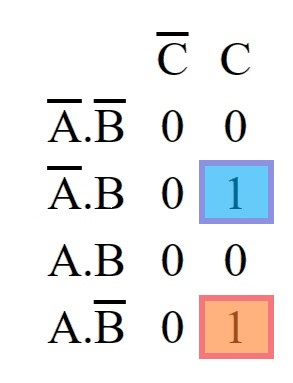
\includegraphics[scale=1]{figures/e3_tp3_ej3_moore_y0_kmap.jpg}
	\caption{$Y_0$ Karnaugh map}
\end{figure}

\begin{figure}[H]
	\centering
	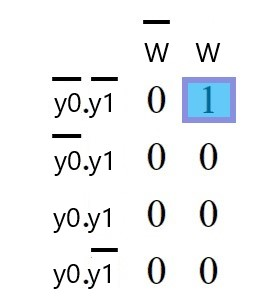
\includegraphics[scale=1]{figures/e3_tp3_ej3_moore_y1_kmap.jpg}
	\caption{$Y_1$ Karnaugh map}
\end{figure}

\begin{figure}[H]
	\centering
	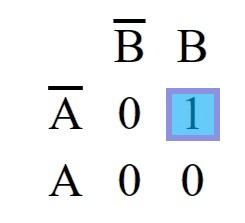
\includegraphics[scale=0.9]{figures/e3_tp3_ej3_moore_z_kmap.jpg}
	\caption{$Z$ Karnaugh map}
\end{figure}

\subsection{Outputs and next states schematics}
\begin{figure}[H]
	\centering
	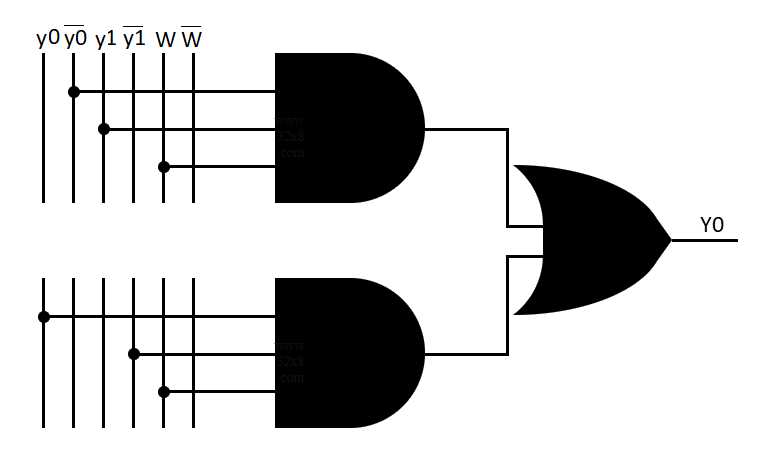
\includegraphics{figures/ej3_Y0_schem_moore.PNG}
	\caption{$Y_0$ schematic as a sum-of-products}
\end{figure}
\begin{figure}[H]
	\centering
	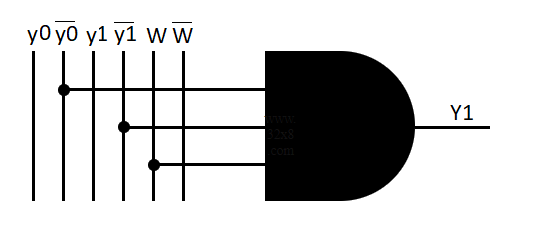
\includegraphics{figures/ej3_Y1_schem_moore.PNG}
	\caption{$Y_1$ schematic as a sum-of-products}
\end{figure}
\begin{figure}[H]
	\centering
	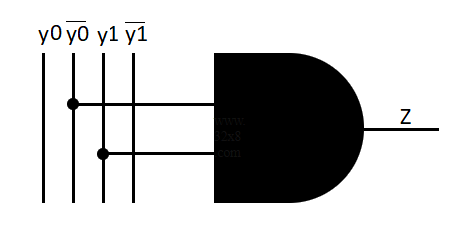
\includegraphics{figures/ej3_Z_schem_moore.PNG}
	\caption{$Y_2$ schematic as a sum-of-products}
\end{figure}



\section{Mealy-type FSM implementation}
\subsection{FSM flow-chart}
\begin{figure}[H]
	\centering
	\begin{tikzpicture}
	\begin{pgfonlayer}{nodelayer}
		\node [style=estado] (0) at (-6.5, 2) {Pump 1 only};
		\node [style=estado] (1) at (6.5, 2) {Next single pump: 2};
		\node [style=estado] (3) at (-6.5, -2.325) {Next single pump: 1};
		\node [style=estado] (4) at (6.5, -2.325) {Pump 2 only};
		\node [style=none] (5) at (6.5, 1.25) {};
		\node [style=none] (6) at (6.5, -1.575) {};
		\node [style=none] (7) at (6.5, -1.575) {};
		\node [style=none] (8) at (-6.5, 1.25) {};
		\node [style=none] (9) at (-6.5, -1.575) {};
		\node [style=none] (19) at (0, -4.75) {I=S=1 / A=B=0};
		\node [style=none] (20) at (0, -3.25) {I=S=0 / A=B=1};
		\node [style=none] (25) at (-5, 0.25) {I=1, S=0};
		\node [style=none] (26) at (5.25, 0.25) {I=1, S=0};
		\node [style=none] (28) at (-5, -0.575) {A=1, B=0};
		\node [style=none] (30) at (5.25, -0.575) {A=0, B=1};
		\node [style=none] (35) at (7.25, -3) {};
		\node [style=none] (36) at (5, -5) {};
		\node [style=none] (37) at (5.75, -3) {};
		\node [style=none] (38) at (5, -3.625) {};
		\node [style=none] (39) at (-5, -5.05) {};
		\node [style=none] (40) at (-7, -2.9) {};
		\node [style=none] (41) at (-5, -3.65) {};
		\node [style=none] (42) at (-5.625, -2.9) {};
		\node [style=none] (43) at (0, 5.25) {I=S=1 / A=B=0};
		\node [style=none] (44) at (0, 3.75) {I=S=0 / A=B=1};
		\node [style=none] (45) at (-7.25, 2.75) {};
		\node [style=none] (46) at (-5, 4.75) {};
		\node [style=none] (47) at (-5.75, 2.75) {};
		\node [style=none] (48) at (-5, 3.375) {};
		\node [style=none] (49) at (5, 4.8) {};
		\node [style=none] (50) at (7, 2.65) {};
		\node [style=none] (51) at (5, 3.4) {};
		\node [style=none] (52) at (5.625, 2.65) {};
	\end{pgfonlayer}
	\begin{pgfonlayer}{edgelayer}
		\draw [style=transicion] (9.center) to (8.center);
		\draw [style=transicion] (5.center) to (7.center);
		\draw [style=transicion, bend left=45] (35.center) to (36.center);
		\draw [style=transicion, bend left=45] (37.center) to (38.center);
		\draw [style=transicion, bend left=45] (39.center) to (40.center);
		\draw [style=transicion, bend left=45] (41.center) to (42.center);
		\draw [style=transicion] (36.center) to (39.center);
		\draw [style=transicion] (38.center) to (41.center);
		\draw [style=transicion, bend left=45] (45.center) to (46.center);
		\draw [style=transicion, bend left=45] (47.center) to (48.center);
		\draw [style=transicion, bend left=45] (49.center) to (50.center);
		\draw [style=transicion, bend left=45, looseness=1.25] (51.center) to (52.center);
		\draw [style=transicion] (46.center) to (49.center);
		\draw [style=transicion] (48.center) to (51.center);
	\end{pgfonlayer}
\end{tikzpicture}

	\caption{Flow diagram for the Mealy-type FSM implementation.}
\end{figure}

\subsection{State descriptions}
\begin{table}[H]	%mealy state descriptions
	\centering
	\begin{tabular}{|c|c|}
	\hline	
	$y_0$  & Description\\	
	\hline 
	0 & The last number detected is a 0\\ 
	\hline 
	1 & The last number detected is a 1\\ 
	\hline 

	\end{tabular} 
	\caption{Possible states for the Mealy-type FSM implementation.}
	\label{tab:ej3_mealy_states}
\end{table}


\subsection{State transition table}
\begin{table}[H]
	\centering
	\begin{tabular}{|c|c|c|}
		\hline 
		state\textbackslash W & 0 & 1 \\ 
		\hline 
		0 & 0/0 & 1/1 \\ 
		\hline 
		1 & 0/0 & 1/0 \\ 
		\hline 
	\end{tabular} 
	\caption[States transitions and outputs for the Mealy-type FSM implementation]{States transitions and outputs for the Mealy-type FSM implementation. Each cell has the format $next\, state\, / \, Z$}
	\label{tab:ej3_mealy_transitions}
\end{table}

\subsection{Outputs and next states Karnaugh maps}

\begin{figure}[H]
	\centering
	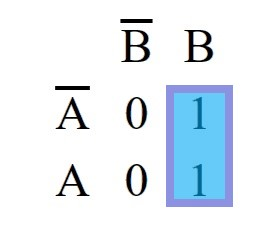
\includegraphics[scale=1]{figures/e3_tp3_ej3_mealy_y0_kmap.jpg}
	\caption{$Y_0$ Karnaugh map}
\end{figure}

\begin{figure}[H]
	\centering
	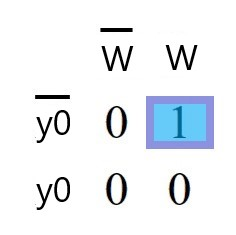
\includegraphics[scale=1]{figures/e3_tp3_ej3_mealy_z_kmap.jpg}
	\caption{$Z$ Karnaugh map}
\end{figure}


\subsection{Output and next states schematics}
\begin{figure}[H]
	\centering
	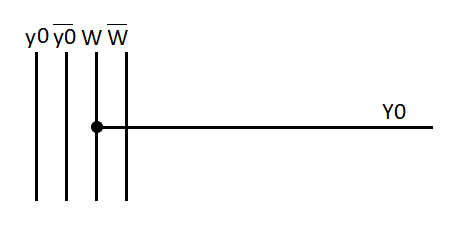
\includegraphics{figures/ej3_Y0_schem_mealy.PNG}
	\caption{$Y_0$ schematic as a sum-of-products}
\end{figure}
\begin{figure}[H]
	\centering
	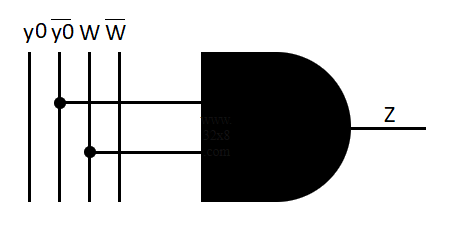
\includegraphics{figures/ej3_Z_schem_mealy.PNG}
	\caption{$Z$ schematic as a sum-of-products}
\end{figure}


\end{document}
